% answers.tex —— 2012 年·全国大纲卷·理科 · 参考答案与详细解析片段
% 由 tools/generate_projects.py 依来源总账自 2012/2012_数学真题_全国大纲理_试题.md + 2012/2012_数学真题_全国大纲理_解析正文.md + 2012/2012_数学真题_全国大纲理_答案要点.md 生成，勿手改（改源 MD 后重跑）


\begin{answer}
\gksolhead{1}{}

\textbf{题目}：

复数 $\dfrac{-1+3i}{1+i}=$\mbox{（　　）}

\begin{gkopts}(4)
\task （A）$2+i$
\task （B）$2-i$
\task （C）$1+2i$
\task （D）$1-2i$
\end{gkopts}

\Needspace{4\baselineskip}
\textbf{解析}

\Needspace{5\baselineskip}
分子分母同乘 $1-i$，得
\nopagebreak[4]
\[
\frac{-1+3i}{1+i}=\frac{(-1+3i)(1-i)}2=1+2i.
\]
故选 C。

\gkanswer{答案：C}

\end{answer}
\begin{answer}
\gksolhead{2}{}

\textbf{题目}：

已知集合 $A=\{1,3,\sqrt m\}$，$B=\{1,m\}$，$A\cup B=A$，则 $m=$\mbox{（　　）}

\begin{gkopts}(2)
\task （A）$0$ 或 $\sqrt3$
\task （B）$0$ 或 $3$
\task （C）$1$ 或 $\sqrt3$
\task （D）$1$ 或 $3$
\end{gkopts}

\Needspace{4\baselineskip}
\textbf{解析}

$A\cup B=A$ 等价于 $B\subseteq A$，所以 $m\in\{1,3,\sqrt m\}$。按题面把 $A$ 写成三个元素的通常约定，$m=1$ 会使 $1$ 与 $\sqrt m$ 重合，不计入该三元素集合的情形；因此 $m=0$ 或 $m=3$，选 B。

\gksubpart{题面问题 / issue}

题号为 2，固定源印刷页为 725。题面证据为 $A=\{1,3,\sqrt m\}$、$B=\{1,m\}$、$A\cup B=A$。处理方式：按列举项互异的题目惯例，答案为 B（$m=0$ 或 $m=3$）。严格集合语义下，$m=1$ 时 $A=\{1,3\}$、$B=\{1\}$ 也满足 $A\cup B=A$，因此这是题面歧义，不能静默掩盖。

\gkanswer{答案：B}

\end{answer}
\begin{answer}
\gksolhead{3}{}

\textbf{题目}：

椭圆的中心在原点，焦距为 $4$，一条准线为 $x=-4$，则该椭圆的方程为\mbox{（　　）}

（A）$\dfrac{x^2}{16}+\dfrac{y^2}{12}=1$　（B）$\dfrac{x^2}{12}+\dfrac{y^2}{8}=1$

（C）$\dfrac{x^2}{8}+\dfrac{y^2}{4}=1$　（D）$\dfrac{x^2}{12}+\dfrac{y^2}{4}=1$

\Needspace{4\baselineskip}
\textbf{解析}

\Needspace{5\baselineskip}
设椭圆的半长轴为 $a$，半焦距为 $c$。焦距为 $4$，故 $2c=4$，即 $c=2$；准线为 $x=-4$，故 $a^2/c=4$，从而 $a^2=8$。于是 $b^2=a^2-c^2=4$，椭圆方程为
\nopagebreak[4]
\[
\frac{x^2}{8}+\frac{y^2}{4}=1.
\]
选 C。

\gkanswer{答案：C}

\end{answer}
\begin{answer}
\gksolhead{4}{}

\textbf{题目}：

已知正四棱柱 $ABCD-A_1B_1C_1D_1$ 中，$AB=2$，$CC_1=2\sqrt2$，$E$ 为 $CC_1$ 的中点，则直线 $AC_1$ 到平面 $BED$ 的距离为\mbox{（　　）}

\begin{gkopts}(4)
\task （A）$2$
\task （B）$\sqrt3$
\task （C）$\sqrt2$
\task （D）$1$
\end{gkopts}

\Needspace{4\baselineskip}
\textbf{解析}

\Needspace{5\baselineskip}
取
\nopagebreak[4]
\[
A=(0,0,0),\quad B=(2,0,0),\quad C=(2,2,0),\quad D=(0,2,0),
\]
\nopagebreak[4]
\[
C_1=(2,2,2\sqrt2),\quad E=(2,2,\sqrt2).
\]
\Needspace{5\baselineskip}
平面 $BED$ 的一个法向量可取 $(\sqrt2,\sqrt2,-2)$，其方程为
\nopagebreak[4]
\[
\sqrt2(x-2)+\sqrt2y-2z=0.
\]
\Needspace{5\baselineskip}
直线 $AC_1$ 的方向向量为 $(2,2,2\sqrt2)$，与该法向量的内积为 $0$，所以直线平行于平面。代入点 $A$，距离为
\nopagebreak[4]
\[
\frac{2\sqrt2}{\sqrt{2+2+4}}=1.
\]
选 D。

\gkanswer{答案：D}

\end{answer}
\begin{answer}
\gksolhead{5}{}

\textbf{题目}：

已知等差数列 $\{a_n\}$ 前 $n$ 项和为 $S_n$．$a_5=5$，$S_5=15$，则数列 $\left\{\dfrac1{a_na_{n+1}}\right\}$ 的前 $100$ 项和为\mbox{（　　）}

\begin{gkopts}(2)
\task （A）$\dfrac{100}{101}$
\task （B）$\dfrac{99}{101}$
\task （C）$\dfrac{99}{100}$
\task （D）$\dfrac{101}{100}$
\end{gkopts}

\Needspace{4\baselineskip}
\textbf{解析}

\Needspace{5\baselineskip}
由等差数列求和公式，
\nopagebreak[4]
\[
15=S_5=\frac{5(a_1+a_5)}2=\frac{5(a_1+5)}2,
\]
\Needspace{5\baselineskip}
得 $a_1=1$。又 $a_5=a_1+4d=5$，所以 $d=1$，即 $a_n=n$。因此
\nopagebreak[4]
\[
\sum_{n=1}^{100}\frac1{a_na_{n+1}}
=\sum_{n=1}^{100}\frac1{n(n+1)}
=\sum_{n=1}^{100}\left(\frac1n-\frac1{n+1}\right)
=\frac{100}{101}.
\]
选 A。

\gkanswer{答案：A}

\end{answer}
\begin{answer}
\gksolhead{6}{}

\textbf{题目}：

$\triangle ABC$ 中，$AB$ 边的高为 $CD$，若 $\overrightarrow{CB}=\boldsymbol a$，$\overrightarrow{CA}=\boldsymbol b$，$\boldsymbol a\cdot\boldsymbol b=0$，$|\boldsymbol a|=1$，$|\boldsymbol b|=2$，则 $\overrightarrow{AD}=$\mbox{（　　）}

\begin{gkopts}(1)
\task （A）$\dfrac13\boldsymbol a-\dfrac13\boldsymbol b$
\task （B）$\dfrac23\boldsymbol a-\dfrac23\boldsymbol b$
\task （C）$\dfrac35\boldsymbol a-\dfrac35\boldsymbol b$
\task （D）$\dfrac45\boldsymbol a-\dfrac45\boldsymbol b$
\end{gkopts}

\Needspace{4\baselineskip}
\textbf{解析}

\Needspace{5\baselineskip}
以 $C$ 为原点，则 $B=\boldsymbol a$、$A=\boldsymbol b$。设 $D=A+t(B-A)$，因 $CD\perp AB$，有
\nopagebreak[4]
\[
\bigl(\boldsymbol b+t(\boldsymbol a-\boldsymbol b)\bigr)\cdot(\boldsymbol a-\boldsymbol b)=0.
\]
\Needspace{5\baselineskip}
利用 $\boldsymbol a\cdot\boldsymbol b=0$、$|\boldsymbol a|=1$、$|\boldsymbol b|=2$，得 $-4+5t=0$，即 $t=\dfrac45$。故
\nopagebreak[4]
\[
\overrightarrow{AD}=t(\boldsymbol a-\boldsymbol b)=\frac45\boldsymbol a-\frac45\boldsymbol b.
\]
选 D。

\gkanswer{答案：D}

\end{answer}
\begin{answer}
\gksolhead{7}{}

\textbf{题目}：

已知 $\alpha$ 为第二象限角，$\sin\alpha+\cos\alpha=\dfrac{\sqrt3}{3}$，则 $\cos2\alpha=$\mbox{（　　）}

\begin{gkopts}(2)
\task （A）$-\dfrac{\sqrt5}{3}$
\task （B）$-\dfrac{\sqrt5}{9}$
\task （C）$\dfrac{\sqrt5}{9}$
\task （D）$\dfrac{\sqrt5}{3}$
\end{gkopts}

\Needspace{4\baselineskip}
\textbf{解析}

\Needspace{5\baselineskip}
由
\nopagebreak[4]
\[
\left(\sin\alpha+\cos\alpha\right)^2=1+\sin2\alpha=\frac13,
\]
\Needspace{5\baselineskip}
得 $\sin2\alpha=-\dfrac23$。又 $\alpha$ 为第二象限角，故 $2\alpha\in(\pi,2\pi)$，且由 $\sin\alpha+\cos\alpha>0$ 可知 $\cos2\alpha<0$。于是
\nopagebreak[4]
\[
\cos2\alpha=-\sqrt{1-\frac49}=-\frac{\sqrt5}{3}.
\]
选 A。

\gkanswer{答案：A}

\end{answer}
\begin{answer}
\gksolhead{8}{}

\textbf{题目}：

已知 $F_1\text{、}F_2$ 为双曲线 $C:x^2-y^2=2$ 的左、右焦点，点 $P$ 在 $C$ 上，$|PF_1|=2|PF_2|$，则 $\cos\angle F_1PF_2=$\mbox{（　　）}

\begin{gkopts}(4)
\task （A）$\dfrac14$
\task （B）$\dfrac35$
\task （C）$\dfrac34$
\task （D）$\dfrac45$
\end{gkopts}

\Needspace{4\baselineskip}
\textbf{解析}

\Needspace{5\baselineskip}
双曲线 $x^2-y^2=2$ 中 $a^2=2$、$c^2=4$，所以 $F_1F_2=2c=4$。设 $|PF_2|=u$，则 $|PF_1|=2u$，而双曲线焦半径之差为 $2a=2$，故 $u=2$。在三角形 $F_1PF_2$ 中用余弦定理：
\nopagebreak[4]
\[
\cos\angle F_1PF_2=\frac{4^2+2^2-4^2}{2\cdot4\cdot2}=\frac14.
\]
选 A。

\gkanswer{答案：A}

\end{answer}
\begin{answer}
\gksolhead{9}{}

\textbf{题目}：

已知 $x=\ln\pi$，$y=\log_5 2$，$z=\mathrm e^{-\frac12}$，则\mbox{（　　）}

\begin{gkopts}(4)
\task （A）$x<y<z$
\task （B）$z<x<y$
\task （C）$z<y<x$
\task （D）$y<z<x$
\end{gkopts}

\Needspace{4\baselineskip}
\textbf{解析}

\Needspace{5\baselineskip}
有 $\ln\pi>1$，$\log_52<1$，且 $\mathrm e^{-1/2}<1$。直接比较可得
\nopagebreak[4]
\[
\log_52<\mathrm e^{-1/2}<\ln\pi,
\]
故选 D。

\gkanswer{答案：D}

\end{answer}
\begin{answer}
\gksolhead{10}{}

\textbf{题目}：

已知函数 $y=x^3-3x+c$ 的图象与 $x$ 轴恰有两个公共点，则 $c=$\mbox{（　　）}

\begin{gkopts}(2)
\task （A）$-2$ 或 $2$
\task （B）$-9$ 或 $3$
\task （C）$-1$ 或 $1$
\task （D）$-3$ 或 $1$
\end{gkopts}

\Needspace{4\baselineskip}
\textbf{解析}

\Needspace{5\baselineskip}
令 $g(x)=x^3-3x+c$，则 $g'(x)=3(x^2-1)$，极值点为 $x=-1,1$。图象与 $x$ 轴恰有两个公共点时，必有一个极值点在 $x$ 轴上，即
\nopagebreak[4]
\[
g(-1)=c+2=0\quad\text{或}\quad g(1)=c-2=0.
\]
所以 $c=-2$ 或 $2$，选 A。

\gkanswer{答案：A}

\end{answer}
\begin{answer}
\gksolhead{11}{}

\textbf{题目}：

将字母 $a,a,b,b,c,c$ 排成三行两列，要求每行的字母互不相同，每列的字母也互不相同，则不同的排列方法共有\mbox{（　　）}

\begin{gkopts}(4)
\task （A）$12$ 种
\task （B）$18$ 种
\task （C）$24$ 种
\task （D）$36$ 种
\end{gkopts}

\Needspace{4\baselineskip}
\textbf{解析}

\Needspace{5\baselineskip}
把六个位置编号为三行两列的格点。每个字母出现两次，且两次不能位于同一行或同一列。将位置划分为三个带标签的二元组，要求每组的两个位置既不同行也不同列。六个位置的无序配对中满足条件的完美配对有 $2$ 个；给三个字母标记的方式有 $3!$ 种。因此排列总数为
\nopagebreak[4]
\[
2\cdot3!=12.
\]
选 A。

\gkanswer{答案：A}

\end{answer}
\begin{answer}
\gksolhead{12}{}

\textbf{题目}：

正方形 $ABCD$ 的边长为 $1$，点 $E$ 在边 $AB$ 上，点 $F$ 在边 $BC$ 上，$AE=BF=\dfrac37$．动点 $P$ 从 $E$ 出发沿直线向 $F$ 运动，每当碰到正方形的边时反弹，反弹时反射角等于入射角，当点 $P$ 第一次碰到 $E$ 时，$P$ 与正方形的边碰撞的次数为\mbox{（　　）}

\begin{gkopts}(4)
\task （A）$16$
\task （B）$14$
\task （C）$12$
\task （D）$10$
\end{gkopts}

\Needspace{4\baselineskip}
\textbf{解析}

\Needspace{5\baselineskip}
将正方形沿边反射展开。取 $A=(0,0)$、$B=(1,0)$、$C=(1,1)$、$D=(0,1)$，则 $E=(3/7,0)$、$F=(1,3/7)$，运动方向的斜率为 $3/4$。展开后运动射线可写成
\nopagebreak[4]
\[
(x,y)=\left(\frac37,0\right)+s(4,3),\quad s>0.
\]
它第一次到达 $E$ 的同像时，$y=6$，且 $x=\dfrac{59}{7}=8+\dfrac37$，对应 $s=2$。途中穿过 $8$ 条竖直网格线和 $6$ 条水平网格线，共碰撞 $14$ 次，选 B。

\gkanswer{答案：B}

\end{answer}
\begin{answer}
\gksolhead{13}{}

\textbf{题目}：

\Needspace{5\baselineskip}
若 $x\text{、}y$ 满足约束条件
\nopagebreak[4]
\[
\begin{cases}
x-y+1\geqslant0,\\
x+y-3\leqslant0,\\
x+3y-3\geqslant0,
\end{cases}
\]
则 $z=3x-y$ 的最小值为\gkblank{}。

\Needspace{4\baselineskip}
\textbf{解析}

\Needspace{5\baselineskip}
约束区域的三个顶点分别为
\nopagebreak[4]
\[
(0,1),\quad(1,2),\quad(3,0).
\]
在三点处 $z=3x-y$ 分别为 $-1,1,9$，所以最小值为 $-1$。

\gkanswer{答案：$-1$}

\end{answer}
\begin{answer}
\gksolhead{14}{}

\textbf{题目}：

当函数 $y=\sin x-\sqrt3\cos x$（$0\leqslant x<2\pi$）取得最大值时，$x=$\gkblank{}。

\Needspace{4\baselineskip}
\textbf{解析}

\nopagebreak[4]
\[
y=\sin x-\sqrt3\cos x=2\sin\left(x-\frac\pi3\right).
\]
\Needspace{5\baselineskip}
在 $[0,2\pi)$ 内取得最大值要求
\nopagebreak[4]
\[
x-\frac\pi3=\frac\pi2,
\]
因此 $x=\dfrac{5\pi}{6}$。

\gkanswer{答案：$\dfrac{5\pi}{6}$}

\end{answer}
\begin{answer}
\gksolhead{15}{}

\textbf{题目}：

若 $\left(x+\dfrac1x\right)^n$ 的展开式中第 3 项与第 7 项的二项式系数相等，则该展开式中 $\dfrac1{x^2}$ 的系数为\gkblank{}。

\Needspace{4\baselineskip}
\textbf{解析}

\Needspace{5\baselineskip}
第 3 项和第 7 项的二项式系数分别为 $\binom n2$、$\binom n6$。由对称性且两下标不同，得 $n-2=6$，所以 $n=8$。展开式通项为
\nopagebreak[4]
\[
\binom8k x^{8-k}x^{-k}=\binom8k x^{8-2k}.
\]
令 $8-2k=-2$，得 $k=5$，故所求系数为 $\binom85=56$。

\gkanswer{答案：$56$}

\end{answer}
\begin{answer}
\gksolhead{16}{}

\textbf{题目}：

三棱柱 $ABC-A_1B_1C_1$ 中，底面边长和侧棱长都相等，$\angle BAA_1=\angle CAA_1=60^\circ$，则异面直线 $AB_1$ 与 $BC_1$ 所成角的余弦值为\gkblank{}。

\Needspace{4\baselineskip}
\textbf{解析}

\Needspace{5\baselineskip}
设底面边长和侧棱长均为 $1$，取
\nopagebreak[4]
\[
A=(0,0,0),\quad B=(1,0,0),\quad C=\left(\frac12,\frac{\sqrt3}{2},0\right).
\]
\Needspace{5\baselineskip}
设 $\overrightarrow{AA_1}=\boldsymbol u$。由题设
\nopagebreak[4]
\[
|\boldsymbol u|=1,\quad \boldsymbol u\cdot\overrightarrow{AB}=\frac12,
\quad \boldsymbol u\cdot\overrightarrow{AC}=\frac12.
\]
\Needspace{5\baselineskip}
从而 $\boldsymbol u=\left(\frac12,\frac1{2\sqrt3},\sqrt{\frac23}\right)$（取相反的竖直方向不影响结果）。于是
\nopagebreak[4]
\[
\overrightarrow{AB_1}=\overrightarrow{AB}+\boldsymbol u,
\quad
\overrightarrow{BC_1}=\overrightarrow{BC}+\boldsymbol u.
\]
\Needspace{5\baselineskip}
计算得
\nopagebreak[4]
\[
\overrightarrow{AB_1}\cdot\overrightarrow{BC_1}=1,
\quad |AB_1|=\sqrt3,
\quad |BC_1|=\sqrt2.
\]
故异面直线所成角的余弦为 $\dfrac1{\sqrt6}=\dfrac{\sqrt6}{6}$。

\gkanswer{答案：$\dfrac{\sqrt6}{6}$}

\end{answer}
\begin{answer}
\gksolhead{17}{}

\textbf{题目}：

$\triangle ABC$ 的内角 $A\text{、}B\text{、}C$ 的对边分别为 $a\text{、}b\text{、}c$，已知 $\cos(A-C)+\cos B=1$，$a=2c$，求 $C$。

\Needspace{4\baselineskip}
\textbf{解析}

\Needspace{5\baselineskip}
由 $A+B+C=\pi$，有
\nopagebreak[4]
\[
\cos(A-C)+\cos B
=2\cos\frac{A-C+B}{2}\cos\frac{A-C-B}{2}
=2\sin C\sin A.
\]
\Needspace{5\baselineskip}
题设给出 $2\sin A\sin C=1$。又由正弦定理和 $a=2c$，得 $\sin A=2\sin C$，所以 $4\sin^2C=1$。因此 $\sin C=\dfrac12$。若 $C=5\pi/6$，则 $A=\pi/2$ 将使 $B<0$，不合三角形条件；故
\nopagebreak[4]
\[
C=\frac\pi6.
\]

\gkanswer{答案：$C=\dfrac\pi6$。}

\end{answer}
\begin{answer}
\gksolhead{18}{}

\textbf{题目}：

如图，四棱锥 $P-ABCD$ 中，底面 $ABCD$ 为菱形，$PA\perp$ 底面 $ABCD$，$AC=2\sqrt2$，$PA=2$，$E$ 是 $PC$ 上的一点，$PE=2EC$。
\nopagebreak[4]
\begin{center}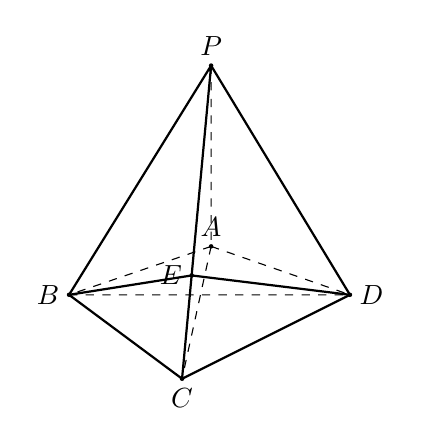
\begin{tikzpicture}[scale=.82,>=stealth]
\coordinate (A) at (0,0);
\coordinate (B) at (-2.2,-.75);
\coordinate (C) at (-.45,-2.05);
\coordinate (D) at (2.15,-.75);
\coordinate (P) at (0,2.8);
\coordinate (E) at (-.3,-.45);

% Visible base edges and lateral edges.
\draw[thick] (B)--(C)--(D);
\draw[thick] (P)--(B) (P)--(C) (P)--(D);
\draw[thick] (E)--(B) (E)--(D);
% Hidden base diagonals/edges and hidden lateral edge.
\draw[dashed] (A)--(B) (A)--(D) (A)--(C) (B)--(D) (P)--(A);
\fill (A) circle (1pt) node[above] {$A$};
\fill (B) circle (1pt) node[left] {$B$};
\fill (C) circle (1pt) node[below] {$C$};
\fill (D) circle (1pt) node[right] {$D$};
\fill (P) circle (1pt) node[above] {$P$};
\fill (E) circle (1pt) node[left] {$E$};
\end{tikzpicture}
\end{center}
\nopagebreak[4]
（1）　证明：$PC\perp$ 平面 $BED$；

（2）　设二面角 $A-PB-C$ 为 $90^\circ$，求 $PD$ 与平面 $PBC$ 所成角的大小。

\Needspace{4\baselineskip}
\textbf{解析}

\Needspace{5\baselineskip}
令底面位于 $z=0$ 平面，取
\nopagebreak[4]
\[
A=(0,0,0),\quad P=(0,0,2),\quad C=(2\sqrt2,0,0),
\]
\nopagebreak[4]
\[
B=(\sqrt2,t,0),\quad D=(\sqrt2,-t,0),
\]
\Needspace{5\baselineskip}
其中 $t\neq0$；此时 $ABCD$ 为菱形且 $AC=2\sqrt2$。由 $PE=2EC$，
\nopagebreak[4]
\[
E=\frac13P+\frac23C=\left(\frac{4\sqrt2}{3},0,\frac23\right).
\]
\Needspace{5\baselineskip}
于是 $\overrightarrow{PC}=(2\sqrt2,0,-2)$，而
\nopagebreak[4]
\[
\overrightarrow{EB}=\left(-\frac{\sqrt2}{3},t,-\frac23\right),
\quad
\overrightarrow{ED}=\left(-\frac{\sqrt2}{3},-t,-\frac23\right).
\]
\gksubpart{(1)}

直接计算得 $\overrightarrow{PC}\cdot\overrightarrow{EB}=\overrightarrow{PC}\cdot\overrightarrow{ED}=0$。因 $EB\text{、}ED$ 是平面 $BED$ 内的两条相交直线，故 $PC\perp$ 平面 $BED$。

\gksubpart{(2)}

\Needspace{5\baselineskip}
再考虑二面角条件。由平面 $APB$、$CPB$ 的法向量可分别取
\nopagebreak[4]
\[
\boldsymbol n_1=(-t,\sqrt2,0),
\quad
\boldsymbol n_2=(t,\sqrt2,\sqrt2t).
\]
\Needspace{5\baselineskip}
二面角为 $90^\circ$ 等价于 $\boldsymbol n_1\cdot\boldsymbol n_2=0$，故 $t^2=2$。不妨取 $t=\sqrt2$，则平面 $PBC$ 的一个法向量为 $(\sqrt2,\sqrt2,2)$，而
\nopagebreak[4]
\[
\overrightarrow{PD}=(\sqrt2,-\sqrt2,-2).
\]
\Needspace{5\baselineskip}
设 $PD$ 与平面 $PBC$ 所成角为 $\theta$，则
\nopagebreak[4]
\[
\sin\theta
=\frac{|\overrightarrow{PD}\cdot(\sqrt2,\sqrt2,2)|}
{|\overrightarrow{PD}|\,|(\sqrt2,\sqrt2,2)|}
=\frac4{(2\sqrt2)(2\sqrt2)}=\frac12.
\]
所以 $\theta=30^\circ$。

\gkanswer{答案（1）：见解析版}

\gkanswer{答案（2）：$PD$ 与平面 $PBC$ 所成角为 $30^\circ$。}

\end{answer}
\begin{answer}
\gksolhead{19}{}

\textbf{题目}：

乒乓球比赛规则规定：一局比赛，双方比分在 $10$ 平前，一方连续发球 $2$ 次后，对方再连续发球 $2$ 次，依次轮换。每次发球，胜方得 $1$ 分，负方得 $0$ 分。设在甲、乙的比赛中，每次发球，发球方得 $1$ 分的概率为 $0.6$，各次发球的胜负结果相互独立。甲、乙的一局比赛中，甲先发球。

（1）　求开始第 $4$ 次发球时，甲、乙的比分为 $1$ 比 $2$ 的概率；

（2）　$\xi$ 表示开始第 $4$ 次发球时乙的得分，求 $\xi$ 的期望。

\Needspace{4\baselineskip}
\textbf{解析}

开始第 $4$ 次发球前，前两次由甲发球，第 $3$ 次由乙发球。记得分归属于发球方的概率为 $0.6$。

\gksubpart{(1)}

\Needspace{5\baselineskip}
若前两次甲得 $0$ 分，则第 $3$ 次甲得 $1$ 分；若前两次甲得 $1$ 分，则第 $3$ 次甲不得分。因此所求概率为
\nopagebreak[4]
\[
(0.4)^2\cdot0.4+\binom21(0.6)(0.4)\cdot0.6
=0.352=\frac{44}{125}.
\]

\gksubpart{(2)}

\Needspace{5\baselineskip}
乙在前两次甲发球中的期望得分为 $2\times0.4$，第 $3$ 次乙发球时的期望得分为 $0.6$。由期望的线性性质，
\nopagebreak[4]
\[
E(\xi)=2\times0.4+0.6=1.4=\frac75.
\]

\gkanswer{答案（1）：$\dfrac{44}{125}$}

\gkanswer{答案（2）：$E(\xi)=\dfrac75$}

\end{answer}
\begin{answer}
\gksolhead{20}{}

\textbf{题目}：

设函数 $f(x)=ax+\cos x$，$x\in[0,\pi]$。

（1）　讨论 $f(x)$ 的单调性；

（2）　设 $f(x)\leqslant1+\sin x$，求 $a$ 的取值范围。

\Needspace{4\baselineskip}
\textbf{解析}

\gksubpart{(1)}

$f'(x)=a-\sin x$。

当 $a\leqslant0$ 时，$f'(x)\leqslant0$，且除端点外严格为负，故 $f$ 在 $[0,\pi]$ 上单调递减。

当 $0<a<1$ 时，令 $\alpha=\arcsin a\in(0,\pi/2)$，则 $f'$ 在 $\alpha$、$\pi-\alpha$ 处为零，符号依次为正、负、正，所以 $f$ 在 $[0,\alpha]$、$[\pi-\alpha,\pi]$ 上递增，在 $[\alpha,\pi-\alpha]$ 上递减。

当 $a\geqslant1$ 时，$f'(x)\geqslant0$，故 $f$ 在 $[0,\pi]$ 上单调递增。

\gksubpart{(2)}

\Needspace{5\baselineskip}
题设不等式等价于
\nopagebreak[4]
\[
a\leqslant\frac{1+\sin x-\cos x}{x}\quad(0<x\leqslant\pi).
\]
\Needspace{5\baselineskip}
在 $x=\pi$ 处得到必要条件 $a\leqslant2/\pi$。反之，令
\nopagebreak[4]
\[
h(x)=1+\sin x-\cos x-\frac{2x}{\pi}.
\]
$h(0)=h(\pi)=0$，且 $h'(x)=\sin x+\cos x-2/\pi$ 只有一个位于 $(\pi/2,\pi)$ 的零点；因此 $h$ 先增后减，在整个区间上非负。于是 $a\leqslant2/\pi$ 时原不等式成立，故取值范围为 $a\leqslant2/\pi$。

\gkanswer{答案（1）：当 $a\leqslant0$ 时，$f$ 在 $[0,\pi]$ 上单调递减；当 $0<a<1$ 时，令 $\alpha=\arcsin a$，则 $f$ 在 $[0,\alpha]$、$[\pi-\alpha,\pi]$ 上递增，在 $[\alpha,\pi-\alpha]$ 上递减；当 $a\geqslant1$ 时，$f$ 在 $[0,\pi]$ 上单调递增。}

\gkanswer{答案（2）：$a\leqslant\dfrac2\pi$}

\end{answer}
\begin{answer}
\gksolhead{21}{}

\textbf{题目}：

已知抛物线 $C:y=(x+1)^2$ 与圆 $M:(x-1)^2+\left(y-\dfrac12\right)^2=r^2$（$r>0$）有一个公共点 $A$，且在 $A$ 处两曲线的切线为同一直线 $l$。

（1）　求 $r$；

（2）　设 $m\text{、}n$ 是异于 $l$ 且与 $C$ 及 $M$ 都相切的两条直线，$m\text{、}n$ 的交点为 $D$，求 $D$ 到 $l$ 的距离。

\Needspace{4\baselineskip}
\textbf{解析}

\gksubpart{(1)}

\Needspace{5\baselineskip}
令抛物线上点的参数为 $t=x+1$，则点为 $(t-1,t^2)$，其切线斜率为 $2t$。圆心为 $O=(1,1/2)$。公共切点处半径垂直于切线，故
\nopagebreak[4]
\[
\bigl((t-1,t^2)-O\bigr)\cdot(1,2t)=0
\]
\Needspace{5\baselineskip}
即 $2t^3-2=0$，所以 $t=1$，公共点 $A=(0,1)$。于是
\nopagebreak[4]
\[
r=|AO|=\sqrt{(-1)^2+\left(\frac12\right)^2}=\frac{\sqrt5}{2},
\quad l:y=2x+1.
\]

\gksubpart{(2)}

\Needspace{5\baselineskip}
抛物线在参数 $t$ 处的切线为
\nopagebreak[4]
\[
L_t:y=2tx+2t-t^2.
\]
\Needspace{5\baselineskip}
它与圆相切的条件是圆心到该直线的距离等于 $r$，即
\nopagebreak[4]
\[
\frac{|{-t^2+4t-1/2}|}{\sqrt{4t^2+1}}=\frac{\sqrt5}{2}.
\]
\Needspace{5\baselineskip}
化简得
\nopagebreak[4]
\[
t^4-8t^3+12t^2-4t-1=0
=(t-1)^2(t^2-6t-1)=0.
\]
\Needspace{5\baselineskip}
除去 $l$ 对应的 $t=1$，两条直线 $m,n$ 对应的参数为 $u=3+\sqrt{10}$、$v=3-\sqrt{10}$。两条抛物线切线的交点为
\nopagebreak[4]
\[
D=\left(\frac{u+v-2}{2},uv\right)=(2,-1).
\]
\Needspace{5\baselineskip}
故
\nopagebreak[4]
\[
d(D,l)=\frac{|2\cdot2-(-1)+1|}{\sqrt{2^2+(-1)^2}}=\frac6{\sqrt5}=\frac{6\sqrt5}{5}.
\]

\gkanswer{答案（1）：$r=\dfrac{\sqrt5}{2}$}

\gkanswer{答案（2）：$\dfrac6{\sqrt5}=\dfrac{6\sqrt5}{5}$}

\end{answer}
\begin{answer}
\gksolhead{22}{}

\textbf{题目}：

函数 $f(x)=x^2-2x-3$，定义数列 $\{x_n\}$ 如下：

$x_1=2$，$x_{n+1}$ 是过两点 $P(4,5)\text{、}Q_n(x_n,f(x_n))$ 的直线 $PQ_n$ 与 $x$ 轴交点的横坐标。

（1）　证明：$2\leqslant x_n<x_{n+1}<3$；

（2）　求数列 $\{x_n\}$ 的通项公式。

\Needspace{4\baselineskip}
\textbf{解析}

\Needspace{5\baselineskip}
由直线 $PQ_n$ 的 $x$ 轴截距公式，
\nopagebreak[4]
\[
x_{n+1}=\frac{5x_n-4f(x_n)}{5-f(x_n)}.
\]
\Needspace{5\baselineskip}
代入 $f(x)=x^2-2x-3$ 并因式分解，得
\nopagebreak[4]
\[
x_{n+1}=\frac{-4x_n^2+13x_n+12}{8+2x_n-x_n^2}
=\frac{(4-x_n)(4x_n+3)}{(4-x_n)(x_n+2)}
=\frac{4x_n+3}{x_n+2}.
\]

\gksubpart{(1)}

\Needspace{5\baselineskip}
若 $2\leqslant x_n<3$，则
\nopagebreak[4]
\[
x_{n+1}-2=\frac{2x_n-1}{x_n+2}>0,
\quad
3-x_{n+1}=\frac{3-x_n}{x_n+2}>0,
\]
\Needspace{5\baselineskip}
以及
\nopagebreak[4]
\[
x_{n+1}-x_n=\frac{(3-x_n)(x_n+1)}{x_n+2}>0.
\]
由 $x_1=2$ 归纳得 $2\leqslant x_n<x_{n+1}<3$。

\gksubpart{(2)}

\Needspace{5\baselineskip}
令
\nopagebreak[4]
\[
y_n=\frac{x_n-3}{x_n+1}.
\]
\Needspace{5\baselineskip}
则
\nopagebreak[4]
\[
y_{n+1}=\frac{x_{n+1}-3}{x_{n+1}+1}=\frac15y_n,
\quad y_1=-\frac13,
\]
\Needspace{5\baselineskip}
所以 $y_n=-\dfrac1{3\cdot5^{n-1}}$。解回 $x_n$，得
\nopagebreak[4]
\[
x_n=\frac{3+y_n}{1-y_n}
=\frac{9\cdot5^{n-1}-1}{3\cdot5^{n-1}+1}.
\]

\gkanswer{答案（1）：见解析版}

\gkanswer{答案（2）：$x_n=\dfrac{9\cdot5^{n-1}-1}{3\cdot5^{n-1}+1}$}

\end{answer}